\subsection{課題説明}
3種類の連続関数$y=x^2$、$z=x^2+y^2$、$y=-x \times cos(x)$について、
最急降下法の適用を通して探索挙動を観察した。
以下ではまず共通部分である最急降下法の探索手続きについて、
フローチャートを用いて解説する。
その後、3種類の関数毎にプログラムの変更箇所、
観察意図観察方法、観察結果、考察について説明する。


\subsection{Level 2共通部分}

\subsubsection{探索の手続き(フローチャート)}


\begin{figure}[h]
 \begin{center}
  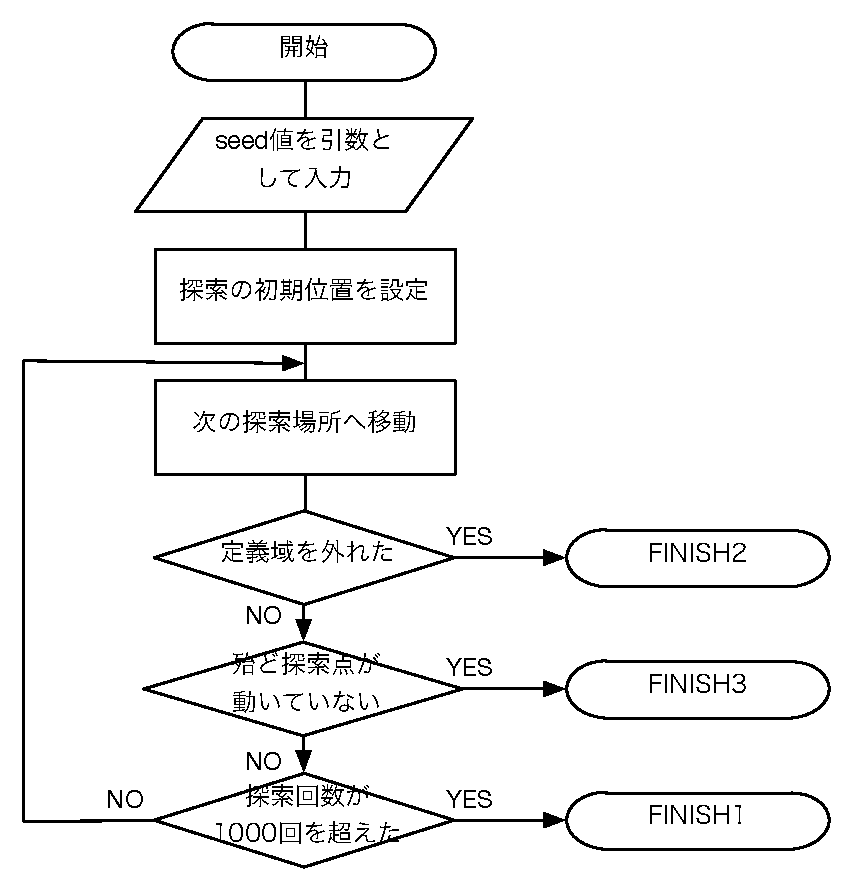
\includegraphics[width=10.0cm]{figs/level2.0/flow.pdf}
  \caption{フローチャート}
	\label{trans_seed}
 \end{center}
\end{figure}


